\section{Sommario}

Abbiamo messo a punto un sistema di rivelazione \emph{multi-purpose} adatto al volo su pallone. Per soddisfare le richieste tecniche ed effettuare tutte le misure di nostro interesse, l'esperimento sfrutta elettronica \emph{ad hoc} e rivelatori alla frontiera tecnologica sviluppati dall'INFN. Prima dell'eventuale lancio testeremo il sistema in laboratorio: questa potrà essere per noi l'occasione di condurre un esperimento di fisica delle particelle, seguendolo in tutte le fasi, dalla progettazione fino all'analisi dati. Le sfide di questo progetto richiedono la collaborazione tra diverse aree del sapere scientifico. La possibilità (e la necessità) di lavorare fianco a fianco fra fisici ed ingegneri per la realizzazione di questo ambizioso progetto di ricerca è un valore aggiunto importante della nostra proposta. Non solo l'esperimento si gioverà della sinergia delle nostre competenze: noi stessi ricaveremo il massimo da questa collaborazione. 

\begin{figure}[h]
\centering
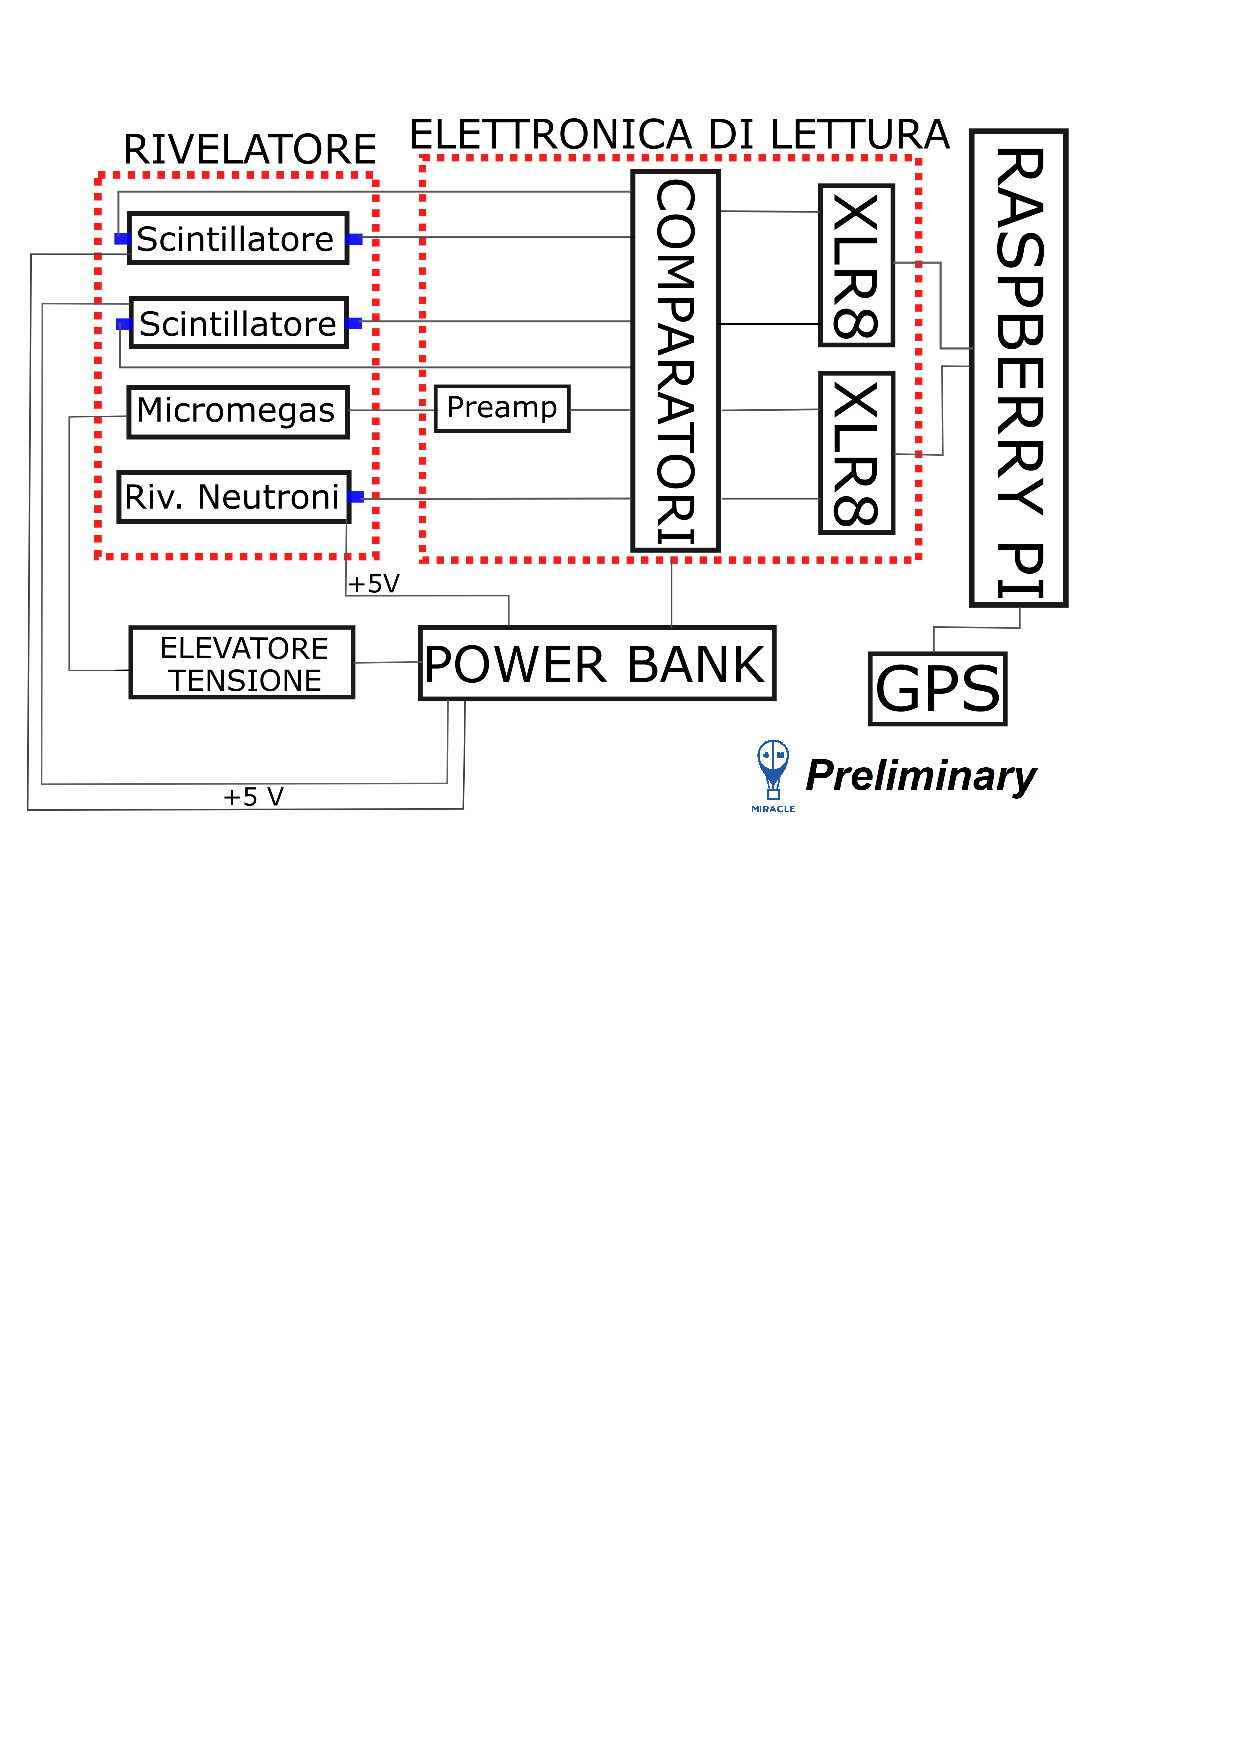
\includegraphics[width=0.5\textwidth]{SCHEMATICA.pdf}
\caption{Schematica riassuntiva dell'apparato rivelatore, dell'elettronica Front-End e dell'elettronica di acquisizioni dati.}
\label{schematica}
\end{figure}
